\chapter[Machine Learning introduction and \emph{N}-fit method development]{Machine Learning introduction and \emph{N}-fit method development}
\label{chap:ml}

%\nota{Comprobar todas las referecnias, meter plots faltantes que en el paper están en el apéndice (siguiente capítulo), comprobar que la escritura tenga sentido (más bien cuando todo acabe) y cambiar el título del capítulo.}


%The $N$-fit reconstruction algorithm is the end product of training a set of supervised deep neural networks (DNNs). In this chapter, we first introduce the Deep Learning tools employed in its configuration along with the innovative use we make of them. Then, we present how we preprocess the input data to the algorithm. Finally, we explain specific details in the development of the $N$-fit algorithm related to results.

The $N$-fit reconstruction algorithm is motivated by a longstanding limitation in ANTARES: for \emph{single-line} (SL) events --typically produced at lower energies-- the standard reconstruction does not provide an azimuthal estimation, leaving the event direction partially unconstrained. Although SL events provide a poorer geometrical baseline than multi-line tracks, they constitute a sizeable fraction of the data at low energy and can be valuable for several physics analyses (e.g., oscillation studies and solar dark-matter searches). Improving their directional reconstruction --particularly recovering azimuthal information-- directly increases the usable statistics and the scientific reach of the detector.

$N$-fit addresses this by training a set of supervised Deep Learning (DL) models tailored to SL topology, aiming to infer direction, event geometry, energy, and class with associated uncertainties. In this chapter, we first introduce the DL tools employed in its design together with the specific, innovative ways we apply them. We then describe the preprocessing pipeline that maps ANTARES data to network inputs. Finally, we detail the development choices behind $N$-fit and present the resulting performance, highlighting the impact on analyses that rely on low-energy SL events.


\section{Deep Learning built-in blocks}
\label{sec:N-fit}

The key feature for the successful performance of the $N$-fit algorithm is the integration of several Deep Learning tools. In this section, we unravel the algorithm: first, we introduce the very basics of artificial neural networks, on which the algorithm is based; then, we describe deep convolutional networks (DCNs) and mixture density networks (MDNs), which play an essential role in $N$-fit's capabilities. Lastly, we describe how we utilized different aspects of transfer learning (TL) to enhance challenging reconstruction analyses, such as energy estimation and event classification.

\subsection{Basics of Artificial Neural Networks}
\label{subsec:ANNs}

Neurons are the core units of neural network models. The basic neuron model in artificial neural networks is the perceptron \cite{perceptron}, which is inspired by the non-linear transduction of synaptic input summation in biological neurons towards action potential firing. Mathematically, the output ($y$) is described as the result of a nonlinear \textit{activation} function of a weighted linear combination of synaptic inputs:

\begin{equation}
	\label{eq:perceptron}
	y = f\left( \sum_i w_i \cdot x_i + b \right) =  f\left( \vec{w}\cdot\vec{x} +b \right),
\end{equation}

where $\vec{x}$, $\vec{w}$, and $b$ represent inputs, weights, and the neuron's bias, respectively. Even though this represents a strong oversimplification of the nonlinear dynamics of biological neurons in the brain, such a computation is capable of mapping arbitrary input-output functions efficiently if multiple perceptrons are present in layers, creating a \textit{feed-forward} network (\autoref{fig:feed-forw}). In $N$-fit, the Rectified Linear Unit \cite{relu} --defined as $\mathrm{ReLU}(x)=\max\{0,x\}$-- is used as the activation function of neurons in the hidden layers.

\begin{figure}[htbp]
	\centering
	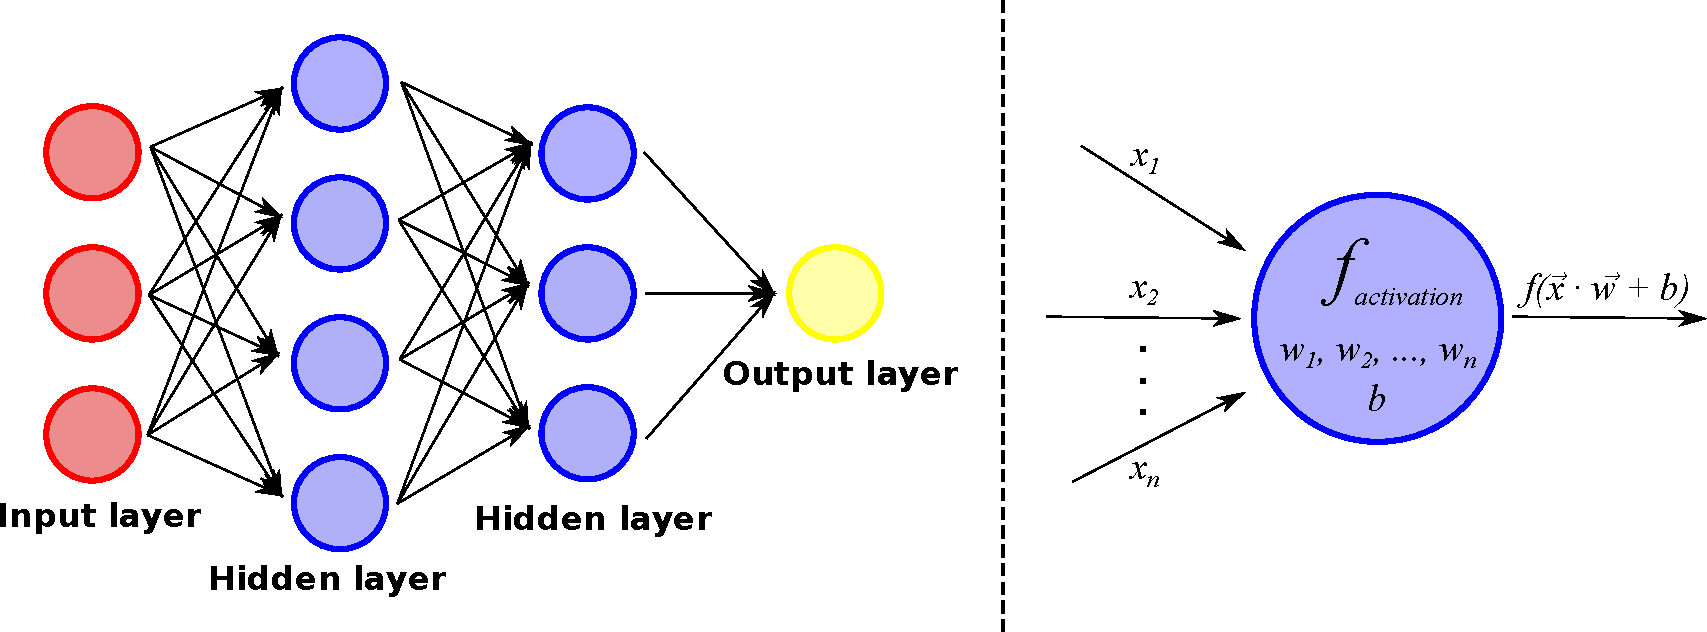
\includegraphics[width=.95\textwidth]{figs2/feed_forward.pdf}
	\caption{\label{fig:feed-forw}Schematic diagram of a simple feed-forward neural network. Circles represent neurons, and arrows represent synaptic connections. In general, more than a single output can be considered.}
\end{figure}


%The final architecture developed for both track and shower events is shown in Figure \ref{fig:network}. The weights initialization was done following Glorot et al. proposal \cite{Glorot} for convolutional layers and He et al. proposal \cite{He} for feed-forward (or dense) layers. To diminish over-fitting during training, we used early stopping \cite{EarlyStop} with a \textit{patience} of 10 epochs, for a maximum of 150. In each epoch, learning batches of 64 input elements were considered. We used the Adam algorithm \cite{Adam} as the learning optimizer because it is able to dynamically regulate the learning rate, which was initialized at $0.001$.


Each layer in the network model processes a level of internal representation that transmits information from one layer to the next. One of the main characteristics of deep vs. shallow learning is precisely its power of abstraction, which is achieved by significantly increasing the number of layers. Data fixes the number of neurons in the input, whereas the number of outputs is concomitant to the question that the model is designed to address. In contrast, the number of hidden layers and the number of neurons in them can vary. These are examples of hyper-parameters that need to be explored while testing the network's performance. Similarly, the learning process is also sensitive to the network's initialization \cite{ini_weights}. We initialized weights and biases randomly following the proposal of He et al. \cite{He} for all the feed-forward layers in the $N$-fit algorithm.

During training in supervised machine learning, the loss function computes the error committed between the network's output and the desired output in data batches (of 64 events in $N$-fit). Weights and biases are updated following error backpropagation, which uses gradient descent to propagate the output loss backwards through the network from the output layer, through the hidden layers, to the input layer. While there are several optimization algorithms based on error backpropagation \cite{SGD}, $N$-fit uses the Adam algorithm \cite{Adam} because it dynamically self-regulates the learning rate, which controls the pace at which learnable parameters in the network adapt. The learning rate was initialized at $0.001$ in every $N$-fit training process.

Typically, the learning procedure iterates over multiple epochs until a predetermined number of cycles is completed, where an epoch constitutes one complete pass of the entire training dataset through the neural network. However, an optimization strategy called Early Stopping enables premature termination of training before reaching this preset epoch threshold in order to diminish the risk of over-fitting \cite{EarlyStop}. This method monitors the loss of the validation dataset after each epoch and halts the process when two conditions are met: the validation loss reaches a minimum value, and a specified number of subsequent epochs (termed the \textit{patience} parameter) elapse without further reduction in validation loss. Upon stopping, the algorithm automatically restores the model parameters corresponding to the optimal validation performance observed during training. We set the maximum number of epochs to 150 and the patience to 10 epochs.

Another technique employed in order to avoid over-fitting is called DropOut \cite{Dropout}. It consists of randomly switching off a preset percentage of random neurons within a layer, so that the active neurons vary in each batch. In this way, DropOut prevents the neurons from becoming too specialised. In the $N$-fit algorithm, 20\% of the neurons from the convolutional block outputs were randomly dropped (i.e. their activation was set to 0) before feeding the first feed-forward layer.


\subsection{Deep Convolutional Networks}
\label{subsec:DCN}

Convolutional neural networks (CCNs) are a class of neural network models designed for processing structured grid data, such as images and image-like tensors \cite{CNN}. Inspired by the human visual system, they are built to recognize patterns and spatial hierarchies efficiently. Unlike traditional fully connected neural networks such as feed-forward ones, which treat every input as independent, CNNs leverage local connectivity, weight sharing, and hierarchical feature extraction to reduce the computational complexity while enhancing learning efficiency. At the heart of a CNN are convolutional layers, which are composed of small, trainable filters that slide over the input image to extract meaningful patterns.  These filters evolve over time through training, adapting to detect increasingly sophisticated features in deeper layers. Initially, filters may identify simple edges or gradients, but as they propagate through deeper layers, they start recognizing textures and shapes. The weight updates are governed by backpropagation and gradient descent, ensuring that the filters become more attuned to distinguishing relevant features from noise. After convolutional operations, the activation function introduces non-linearity to the network. In $N$-fit convolutional layers, ReLU is used, as well as in the fully connected layers. Without the activation function, CNNs would merely perform linear transformations, limiting their ability to capture complex representations.

Pooling layers follow the convolutional layers to refine the feature maps by reducing their spatial dimensions. These layers do not have trainable weights but instead apply fixed operations such as max pooling or average pooling. We used max pooling, the most common method, that retains the most prominent feature in a given region, preserving the strongest activations while discarding less relevant information. This downsampling process helps mitigate overfitting by reducing the number of parameters, thereby improving generalization. By compressing the feature maps, pooling layers also allow subsequent convolutional layers to focus on more abstract features without excessive computational overhead.

Deep Convolutional Networks (DCNs), meaning Deep CNNs, are the main tools used in the development of $N$-fit. DCNs extend traditional CNNs by stacking multiple convolutional, activation, and pooling layers to extract increasingly abstract and hierarchical features from input data. We processed ANTARES data generating image-like tensors that serve as inputs (see \autoref{sec:data}). Weights initialization followed Glorot et al. proposal \cite{Glorot} for every convolutional layer in $N$-fit. 

While basic CNNs can capture low-level patterns such as edges and textures, DCNs leverage deeper architectures to detect complex structures, object parts and entire objects with high accuracy. As the depth increases, feature maps transition from simple to highly abstract representations, enabling superior generalization and performance in tasks like image recognition and object detection. Training DCNs introduces challenges such as vanishing gradients and computational inefficiency. They are addressed through techniques like batch normalization, which we considered in $N$-fit. By deepening the network, DCNs significantly enhance the ability to learn intricate patterns, making them the backbone of state-of-the-art deep learning applications. Lastly, the extracted features from the convolutional layers are fed into fully connected layers, such as those in the feed-forward network explained earlier. At this stage, the network shifts from learning spatial hierarchies to making final predictions. 

\subsection{Mixture Density Networks}
\label{subsec:MDN}

Mixture Density Networks (MDNs) extend traditional regression neural networks by predicting complex, multimodal probability distributions instead of deterministic single-point estimates \cite{MDN}, making them ideal for estimating uncertainty in data. A measure of uncertainty is essential for selecting the most reliable estimates in posterior physics analyses.

The outputs of a MDN model represent the necessary parameters to create the multimodal probability density function from Gaussian kernels. Thus, instead of the typical output $\vec{y}_{p}$ for a single multidimensional prediction, the outputs of the network consist of means $\vec{\mu}_i$, variances $\sigma_i$ and mixture weights $\alpha_i$ (assuming that the outputs are statistically independent):

\begin{equation}
	PDF(\vec{y}_p) = \sum_i^n \alpha_i \cdot N(\vec{\mu}_i, \sigma_i; \vec{y}_p), \quad \quad \text{such that} \quad \sum_i^n \alpha_i = 1,
\end{equation}

where $N(\vec{\mu}, \sigma;\, \vec{y}_p)$ is a multi-dimensional isotropic Gaussian function. The number of Gaussian distributions $n$ must be hand fixed and predicted variances must always be positive, using the appropriate activation function --$N$-fit uses $\text{ELU}+1$ (ELU being the Exponential Linear Unit function). Similarly, the mixture weights use a softmax function to ensure they add to one. The network model learns to predict the parameters of these Gaussians --means, variances, and mixture weights-- using a specialized loss function based on maximum likelihood estimation (MLE), where the network is optimized to maximize the probability of the observed data under the predicted mixture model (\ref{eq:logloss}):

\begin{equation}
	\label{eq:logloss}
	\mathcal{L} = -\ln \left\{ \sum_i^n  \frac{\alpha_i}{(2\pi)^{c/2}\sigma_i^c}\exp\left( -\frac{||\vec{y}_t-\vec{\mu}_i||^2}{2\sigma_i^2} \right) \right\},
\end{equation}

where $c$ is the dimension of the output vector $\vec{y}_t$. In the development of $N$-fit, we only needed to parametrise each of our reconstructed parameters, following each a single Gaussian mode. With $c=1$, the loss function is reduced to:% (\ref{eq:loglossfinal}):

\begin{equation}
	\label{eq:loglossfinal}
	\mathcal{L} = \ln(\sqrt{2\pi}\sigma) + \left( \frac{(y_t-\mu)^2}{2\sigma^2} \right).
\end{equation}

This is different from traditional loss functions like mean-squared error (MSE), as it allows the model to learn distributions that can accommodate multiple correct answers, such as in inverse problems, rather than forcing a single prediction. However, training MDNs can be challenging due to numerical instability, and difficulties in optimizing multiple parameters simultaneously. These effects can be mitigated using regularization techniques, careful initialization strategies, and robust optimization methods like Adam's. In addition to careful initialization and Adam's optimization, $N$-fit avoided numerical instability issues by adding a small contribution to $\sigma$'s activation function: $\text{ELU}+1+\epsilon$. The value $\epsilon = 10^{-5}$ was selected after a quick exploration, in which a balance was achieved between being small enough not to alter the results, but large enough to avoid instability.

By integrating neural networks with probabilistic mixture models, MDNs bridge the gap between deep learning and statistical modelling.

\subsection{Transfer Learning}
\label{subsec:TL}

Transfer learning (TL) refers to the technique of leveraging knowledge gained from previously trained neural network models to improve performance on related tasks \cite{Transfer}. In the context of $N$-fit, we adopt two distinct paradigms of TL: \emph{direct transfer learning}, based on model reuse through layer freezing, and \emph{indirect transfer learning}, relying on knowledge distillation via dimensionality reduction.

% \paragraph{Direct Transfer Learning}

In direct TL, convolutional blocks from pretrained models are reused as fixed feature extractors in subsequent models. Specifically, networks trained for spatial reconstruction are repurposed for classification in $N$-fit between track and shower neutrino events by freezing their convolutional layers. These frozen components are connected in parallel to a feed-forward neural network (FFN), effectively enriching the classifier's input space with spatially encoded representations without requiring retraining of the feature extractors. This strategy benefits from the spatial specialization of each pretrained model and mitigates overfitting by reducing the number of trainable parameters for classification.

% \paragraph{Indirect Transfer Learning via PCA-based Knowledge Distillation}

Indirect TL in $N$-fit is achieved through knowledge distillation \cite{moslemi2024} from pretrained networks by extracting internal activations and transforming them into compact, informative representations using dimensionality reduction techniques. Specifically, this is accomplished using Principal Component Analysis (PCA), a linear dimensionality reduction technique that identifies orthogonal directions (principal components) along which data variability is maximized \cite{PCA}.

PCA is applied to neuron activations from the hidden layers of the networks trained for spatial reconstruction in $N$-fit, which are assumed to encode latent features relevant for energy estimation. These activations form a high-dimensional feature space, potentially redundant or noisy. With the PCA, we can reduce this space by projecting the original activations onto a lower-dimensional subspace defined by the principal components. Components are ordered by their explained variance, and only those contributing significantly to the total variance are retained. This selection ensures that the most informative and least correlated features are preserved.

The resulting low-dimensional vectors serve as inputs to a downstream FFN tasked with energy regression. This setup effectively transfers high-level abstract knowledge learned during direction and distance reconstruction, enabling the energy model to exploit interdependencies among event features not explicitly provided by the original inputs. More generally, this PCA-based approach enables a form of model-agnostic knowledge transfer, where the distilled representations serve as a bridge between pretrained networks and the target model.

Specific details on how Transfer Learning is applied to every reconstruction task are left to \autoref{sec:workflow}.

\section{Dataset preprocessing}
\label{sec:data}

The first step to apply $N$-fit to SL neutrino events was to preprocess the available data as image-like tensors. In this view, the ANTARES telescope is akin to a camera collecting 3D images at each time step, having as many pixels as OMs. For SL events, we created coloured 2D images, with time in one dimension (x-axis) and the storey of the line in the other (y-axis). 
% Creo que esto ya está dicho de antes y rompe el flow.
% Hits refer to detections in OMs that exceeded a threshold. 
The time stamp for each event was relative to the reference hit representing such event, which is the hit that occurred first in time, selected by the $\chi^2$-fit strategy. Next, all hits recorded by the OMs on the line covering a time window of -200 ns to 600 ns relative to the reference hit are selected. Cleaning noisy or background hits is left to the networks themselves. Colours resulted from combining the information provided by the three evenly distributed OMs in each storey. In each pixel of the 2D image, we inserted RGB channels to be informative of the event reconstruction in the horizontal (XY) plane, helping to estimate the azimuthal angle ($\phi$). More specifically, we weighted the angle to which each OM points in XY ($\alpha$) by its recorded voltage amplitudes ($A$). Mathematically, the transformation is represented in equation \ref{eq:RGB}.

\begin{equation}
	\label{eq:RGB}
	(R;G;B) = \left\{
	\begin{aligned}
		A\cdot(1-\tfrac{\alpha}{2\pi/3};\tfrac{\alpha}{2\pi/3};0) ~~~~~~
		\quad\text{if}~~&\alpha \in \left[0, \tfrac{2\pi}{3}\right]
		\\
		A\cdot(0;2-\tfrac{\alpha}{2\pi/3};\tfrac{\alpha}{2\pi/3}-1)
		\quad\text{if}~~&\alpha \in \left[\tfrac{2\pi}{3}, \tfrac{4\pi}{3}\right]
		\\
		A\cdot(\tfrac{\alpha}{2\pi/3}-2;0;3-\tfrac{\alpha}{2\pi/3})
		\quad\text{if}~~&\alpha \in \left[\tfrac{4\pi}{3}, \tfrac{6\pi}{3}\right]
	\end{aligned}
	\right.
\end{equation}

From the discrete hits, we built a continuous signal representing the hit amplitudes over time by applying a Gaussian kernel smoothing with $\sigma = 5$ ns, and then discretized this signal at regular intervals of 5 ns for each individual colour: $\{R(t);G(t);B(t)\}$. Finally, we re-centred the image based on the floor of the reference hit (a representative example is shown in \autoref{fig:RGB}).

Given the huge amount of data available from the ANTARES collaboration, we processed a subset ($\sim$10\%) of MC runs whose identification numbers end in ``0'' in the 2008--2017 period, to keep a good balance between training time and performance. The collected images of SL events were separated into track-like ($\nu_\mu^{CC}$) and shower-like ($\nu_\mu^{NC}$, $\nu_e^{CC}$, $\nu_e^{NC}$) simulations datasets, in order to train specialized models for each event topology. Each dataset was then randomly split in three sub-sets: train (60\%), validation (20\%), and test (20\%). Before feeding images to the network, a Z-score normalization was separately applied to each set. For this, we computed the mean and standard deviation of the respective train sub-sets and applied the transformation to all sub-sets to control for distribution shifts. After the development phase, we also processed other events types, such as simulations of atmospheric muons, random noise background events and real ANATRES data, for control analyses.

\begin{figure}[htbp]
	\centering
	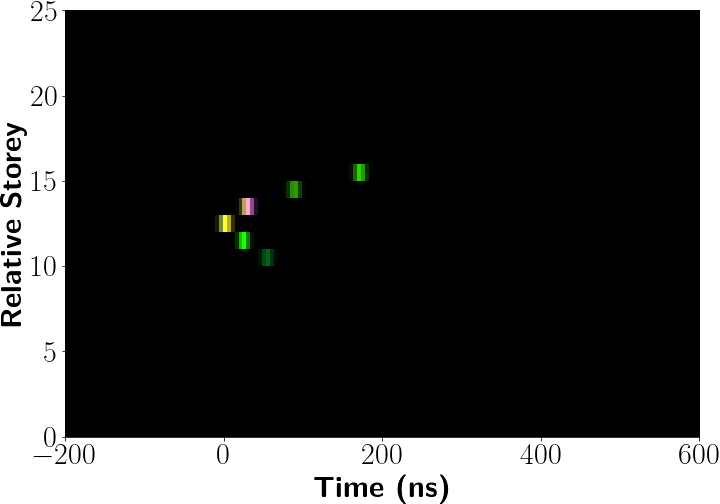
\includegraphics[width=.5\textwidth]{figs2/RGB.png}
	\caption{\label{fig:RGB}Normalized RGB image example of a track event.}
\end{figure}



%%%%%%%%%%%%%%%%%%%%%
%
%
%
%
%
%
%
%
%
%%%%%%%%%%%%%%%%%%%%%%

\section{\emph{N}-fit modular organization}
\label{sec:workflow}

The $N$-fit reconstruction strategy is subdivided into two branches specialized in each type of event: tracks and showers. Each branch cover the different aspects that fully describe neutrino events. The track-branch reconstructs the neutrino direction, the closest point of the secondary muon track to the detector line and the muon energy. Although the shower-branch also reconstructs the direction of the neutrino, it differs slightly in the other parameters, reconstructing the vertex point of the neutrino interaction and its energy. The two branches converge through TL in the classifier that divides the events in tracks or showers. Next subsections explain the details of these network models.

\subsection{Direction reconstruction}
\label{subsec:direction}

%The final architecture developed for both track and shower events is shown in Figure \ref{fig:network}. The weights initialization was done following Glorot et al. proposal \cite{Glorot} for convolutional layers and He et al. proposal \cite{He} for feed-forward (or dense) layers. To diminish over-fitting during training, we used early stopping \cite{EarlyStop} with a \textit{patience} of 10 epochs, for a maximum of 150. In each epoch, learning batches of 64 input elements were considered. We used the Adam algorithm \cite{Adam} as the learning optimizer because it is able to dynamically regulate the learning rate, which was initialized at $0.001$.

Several architectures of increasing complexity were analysed during the optimization of direction reconstruction models for track events. The key steps followed to measure and improve the model's performance are summarised below:

\begin{enumerate}[label={\textit{\roman*})}]
	\item Baseline Control Model: Feed-forward network of four hidden layers implemented to fully reconstruct the Cartesian components of the direction unit vector: $(X;Y;Z)$.
	
	\item Components Separation: Next, the model was divided to reconstruct $Z$ and $\{X,Y\}$ separately. Reconstructions were sequential, first $Z$, then $\{X,Y\}$. We regularized the value of the components $\{X,Y\}$ to penalize deviations of $(X;Y;Z)$ from unit vectors.
	
	\item MDNs and $\theta$ Representation: Point predictions were replaced by inferring probability distributions (MDN). The change did not vary performance but provided event uncertainty estimation, which is of major relevance as a quality metric in posterior physics analyses. Also, the network output $Z$ was replaced by the angle $\theta$, gaining a best estimation of the angle uncertainty, since no error propagation was needed to infer it. %resolution in the limit cases when $Z$ approaches one or minus one. \notaSA{esto último no se acaba de entender}
	
	\item Convolutional Layers: A significant improvement was observed by adding two convolutional layers before the dense network.
	
	\item Image Centring: Aligning events to a centred reference frame further enhanced performance, despite the architecture remained unaltered.
	
	\item Final Adjustments: The number of convolutional layers was optimized (see \autoref{tab:comparison}). From there on, additional layers provided only marginal changes in performance.
	
\end{enumerate}

The progression of the Mean Absolute Error (M.A.E.) through these steps is presented in \autoref{tab:comparison}. The final architecture is illustrated in \autoref{fig:network}. This optimized architecture for the track branch was then applied in the shower branch without further optimization.

% Yo creo que esto no hace falta:
% Additionally, an alternative approach was tested by computing the angle $\phi$ directly instead of $XY$, using techniques for periodic variables, an area where neural networks typically struggle. However, while the resolution remained similar, the reconstructed error did not behave properly. 

% \notaSA{yo añadiría dos filas más para las incertidumbres y allí donde no las contemple la red se  pone  --, así esa ya es de por si una mejora y permite comparar en los casos con los que sí que las contemplan, ya que cuanto menor sea su valor medio mejor, no?} \notaJGM{Lo de las incertidumbres me parece una buena idea, pero ahora mismo no dispongo de esos datos. En los informes originales yo no ponía esa información, de modo que tendrá que ver si tengo las redes entrenadas por ahí o re-entrenar para obtener esa info. Lo dejo como algo que se podría hacer, pero de momento para una primera revisión interna de ANTARES no creo que dé tiempo.}

\begin{table}[htbp]
	\centering
	\renewcommand{\arraystretch}{1.2} % Improves row spacing for better readability
	\begin{tabular}{|c|cc:cccc|}
		\hline
		\textbf{M.A.E.} & \textbf{\textit{i}} & \textbf{\textit{ii}} & \textbf{\textit{iii }} & \textbf{\textit{iv}} & \textbf{\textit{v}} & \textbf{\textit{vi}} \\ \hline
		$\boldsymbol{\theta}$ & $11.2^\circ$ & $10.5^\circ$ & $10.5^\circ$ & $9.6^\circ$ & $8.4^\circ$ & $7.4^\circ$  \\ %\hline
		$\boldsymbol{\phi}$ & $50.1^\circ$ & $49.5^\circ$ & $49.5^\circ$ & $46.2^\circ$ & $44.1^\circ$ & $41.4^\circ$ \\ \hline
	\end{tabular}
	\caption{\label{tab:comparison}Evolution of the Mean Absolute Error (M.A.E.) of the test data set along the key steps followed in the development and optimization of the $N$-fit algorithm for the direction reconstruction of tracks. $\sigma$ estimation was introduced in model (iii).}
\end{table}

\begin{figure}[htbp]
	\centering
	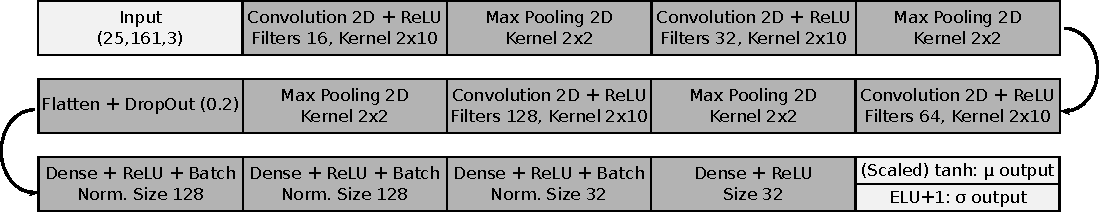
\includegraphics[scale=0.69]{figs2/DCN.pdf}
	\caption{\label{fig:network}Details of the direction neural network architecture. Note that for the $\theta$ prediction, we scaled the hyperbolic tangent activation function for $\mu_\theta$, so that its values lay in $[0, \pi]$ radians. No scaling was necessary for the prediction of $\phi$ since its estimation was derived from the Cartesian $\{X,Y\}$ components of the unit vector.}
\end{figure}

The loss function applied to the angle $\theta$ becomes eq. (\ref{eq:loss_theta}), where $\theta_t$ represents the true value of the angle $\theta$ for each neutrino event in the simulation.

\begin{equation}
	\label{eq:loss_theta}
	\mathcal{L} = \ln (\sqrt{2\pi}\sigma_{\theta}) + \frac{1}{2}\frac{(\theta_{t}-\mu_{\theta} )^2}{\sigma_{\theta}^2},
\end{equation}


A second network predicts the angle $\phi$ through its Cartesian coordinate values ($\mu_X$, $\mu_Y$) and their uncertainties ($\sigma_X$, $\sigma_Y$). The loss function was transformed consequently in equation (\ref{eq:loss_phi}):

%The other network must predict the $\phi$ angle. Since neural networks are inefficient at predicting periodic variables, we used the Cartesian coordinates $XY$ for the $\phi$ reconstruction, as well as their uncertainties. To this end, we used the following loss function:

\begin{equation}
	\label{eq:loss_phi}
	\begin{split}
		\mathcal{L} = &\ln (\sqrt{2\pi}\sigma_{X}) + \frac{1}{2}\frac{(X_{t}-\mu_{X} )^2}{\sigma_{X}^2}+\\
		+ &\ln (\sqrt{2\pi}\sigma_{Y}) + \frac{1}{2}\frac{(Y_{t}-\mu_{Y} )^2}{\sigma_{Y}^2}+\\
		+ &(1-[\mu_{X}^2+\mu_{Y}^2+\cos^2(\mu_{\theta})])^2.
	\end{split}
\end{equation}

The last term in equation (\ref{eq:loss_phi}) regularizes the output of the network, penalizing deviations of $(X;Y;Z)$ from unit vectors. %where the Z component is derived from the $\theta$ prediction as follows: $\mu_Z=\cos(\mu_\theta)$.
To infer the uncertainty of $\phi$, we performed a quadratic error propagation as shown in equation (\ref{eq:error_prop}).

\begin{equation}
	\label{eq:error_prop}
	\sigma_{\phi}^2 = \left(\frac{\partial \phi}{\partial \mu_X}\cdot \sigma_X\right)^2 + \left(\frac{\partial \phi}{\partial \mu_Y}\cdot \sigma_Y\right)^2 \Rightarrow
	\sigma_{\phi} = \frac{\sqrt{\sigma_X^2\cdot \mu_Y^2+\sigma_Y^2\cdot \mu_X^2}}{\mu_X^2+\mu_Y^2 }
\end{equation}

Note that the uncertainty estimation assumes a Gaussian distribution. This means that distribution of errors should become wider although centred with growing $\sigma$ values. For most of the range this is precisely the case when tested, especially for $\theta$ (\autoref{fig:sigma}). As for the uncertainty of the direction reconstruction ($\sigma_{\Omega}$),  we used the expression (\ref{eq:sigma_omega}) derived from the solid angle definition: 

\begin{equation}
	\label{eq:sigma_omega}
	\sigma_\Omega = \sqrt{\sin^2(\theta)\sigma_\phi^2 + \sigma_\theta^2}.
\end{equation}

\begin{figure}[htbp]
	\centering
	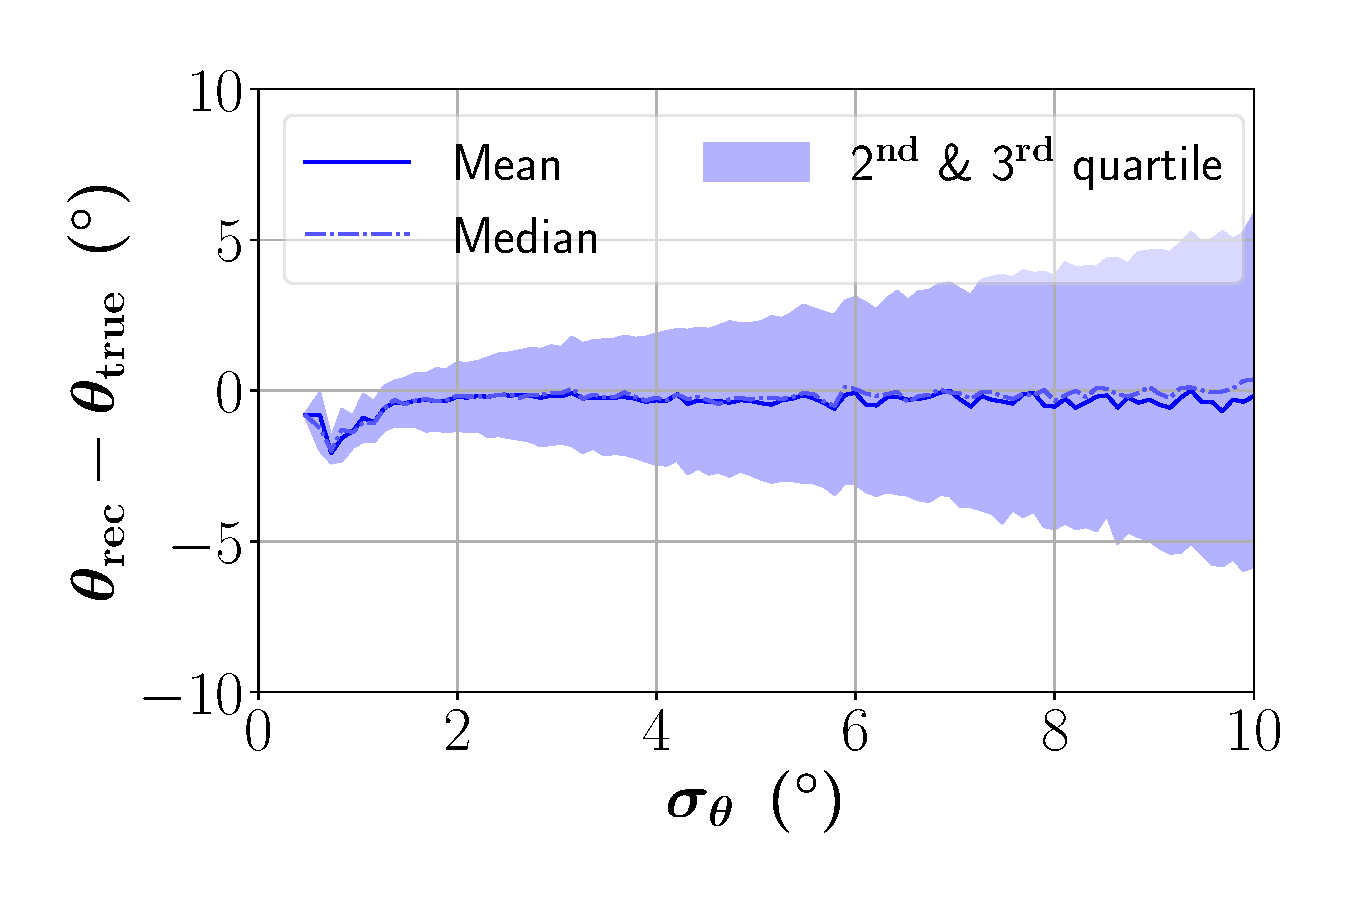
\includegraphics[width=.48\textwidth]{figs2/sigma_Zenith_track}
	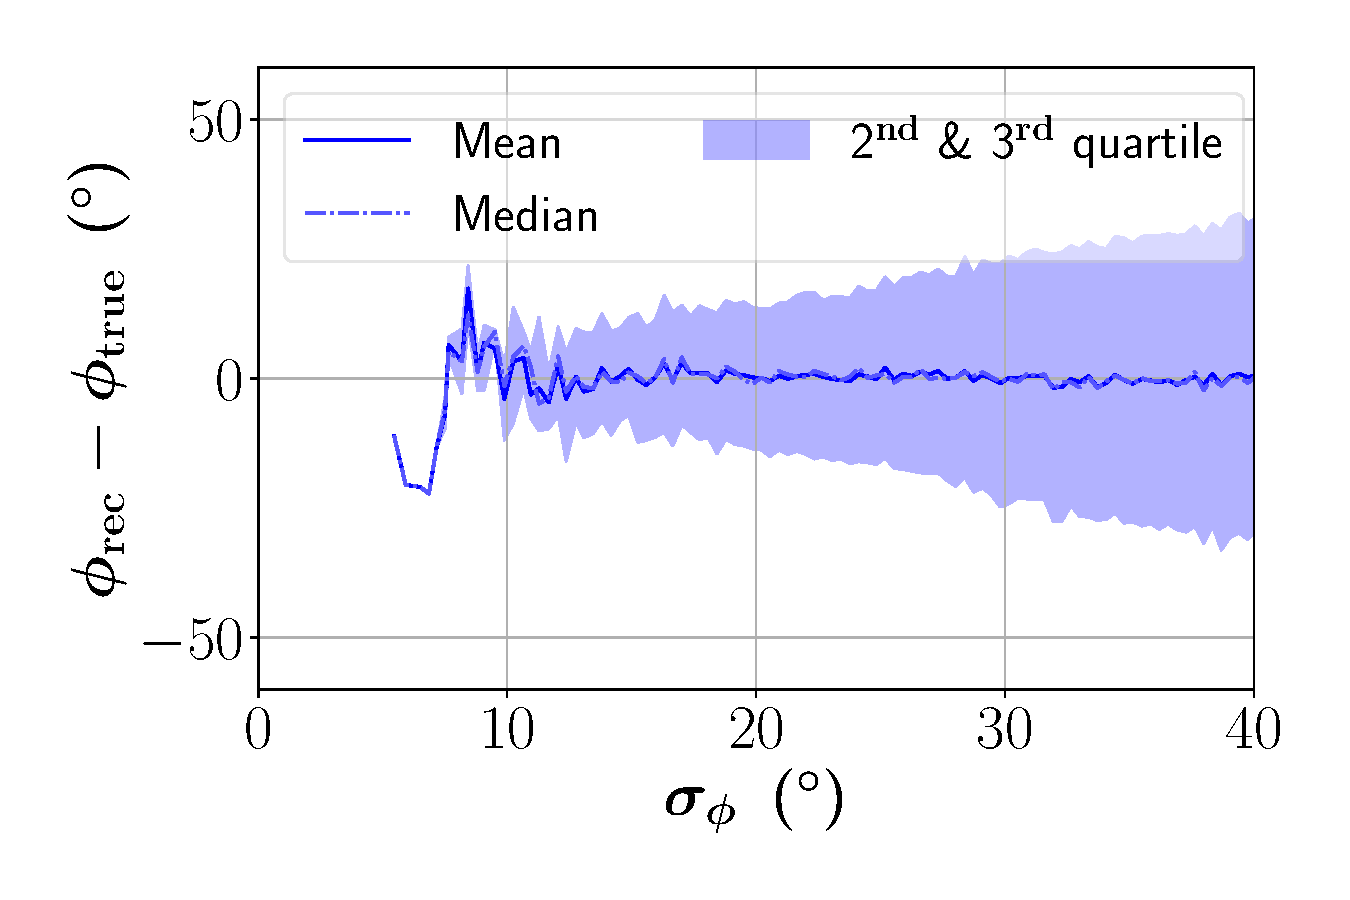
\includegraphics[width=.48\textwidth]{figs2/sigma_Azimuth_track}
	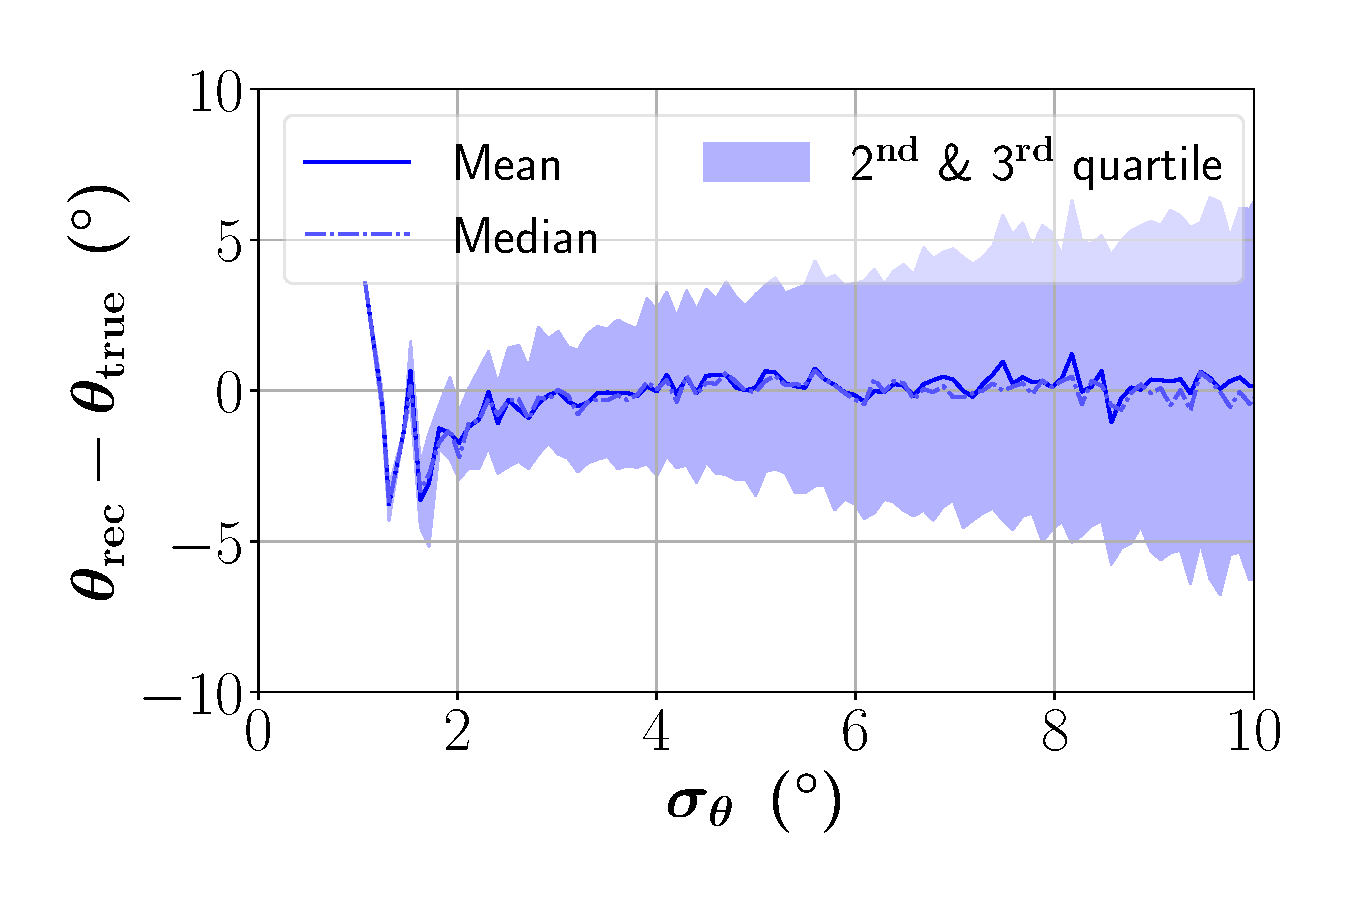
\includegraphics[width=.48\textwidth]{figs2/sigma_Zenith_shower}
	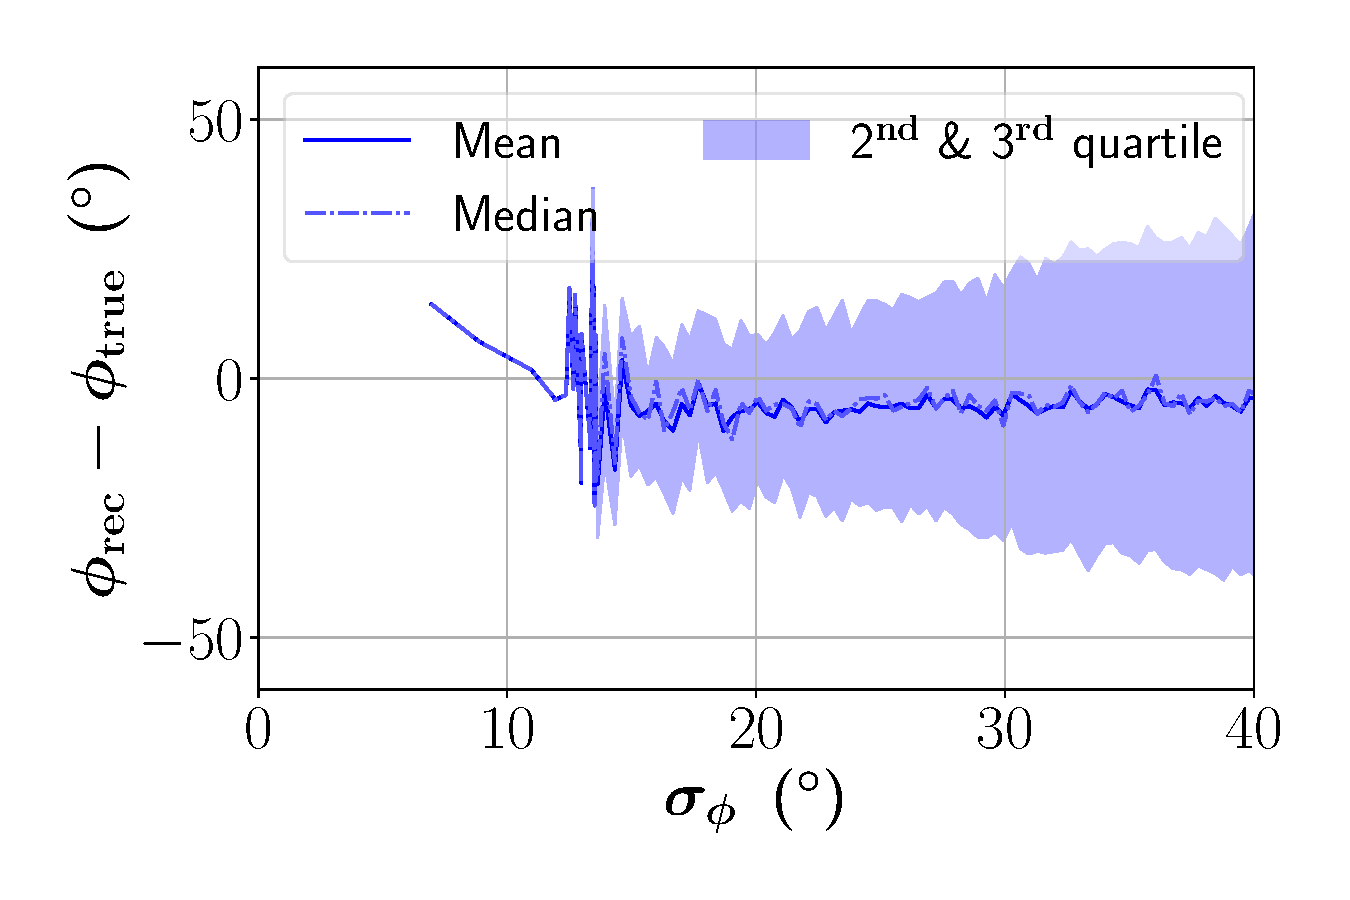
\includegraphics[width=.48\textwidth]{figs2/sigma_Azimuth_shower}
	\caption{\label{fig:sigma}Angles $\theta$ and $\phi$ error as function of the predicted uncertainty for the \textbf{track} (top) and \textbf{shower} (bottom) branches. The mean and median error stay close to zero with no significant bias. Second and third quartiles behave as expected for a Gaussian distribution, especially for $\theta$.}
\end{figure}

%\begin{figure}[htbp]
%	\centering
	
%	\caption{\label{fig:sigma_sh}Angles $\theta$ and $\phi$ error as function of the predicted uncertainty for the \textbf{shower} branch. The mean and median error stay close to zero with no significant bias. Second and third quartiles behave as expected for a Gaussian distribution, especially for $\theta$.}
%\end{figure}



\subsection{Closest point and interaction vertex}
\label{subsec:closest}

%Due to the dependency of the energy deposited in the detector on the distance and position of the event to the lines, we decided to reconstruct these variables before the energy.

In addition to the reconstruction of direction, estimating the energy of neutrino events is fundamental for physics analysis. Energy and distance to the detector are, however, intermingled in SL events: distant high-energy events may appear as SL as much as near low-energy events. Then, to improve the energy estimation, we included in $N$-fit the reconstruction of the \emph{closest point} of track events to the ANTARES detector line, and the \emph{interaction vertex} position of showers events, since these two magnitudes are characterized by the horizontal distance in meters ($R_c$ for closest point of tracks, $R_v$ for interaction vertex of showers) and their vertical position ($Z_c$ for tracks, $Z_v$ for showers) defined in the ANTARES frame of reference.

Independent networks (\autoref{fig:network_RZ}) were used for the horizontal distance ($R$) and vertical coordinate ($Z$). Their architecture was that of the direction reconstruction without further tuning. Differences lay in networks' input and output to fulfil the characteristics of these reconstructions. Thus, events were not centred across images in these network models to ease the reconstruction of $Z$. In addition, these networks also incorporated the reconstruction of $\theta$ as input, which was introduced in parallel to the convolutional layers. Lastly, the loss function, equation (\ref{eq:loss_RZ}), was adapted in consonance with the outputs of these networks: 

\begin{equation}
	\label{eq:loss_RZ}
	\begin{split}
		\mathcal{L} = &\ln (\sqrt{2\pi}\sigma_{R}) + \frac{1}{2}\frac{(R_{t}-\mu_{R} )^2}{\sigma_{R}^2}+\\
		+ &\ln (\sqrt{2\pi}\sigma_{Z}) + \frac{1}{2}\frac{(Z_{t}-\mu_{Z} )^2}{\sigma_{Z}^2}.
	\end{split}
\end{equation}

\begin{figure}[htbp]
	\centering
	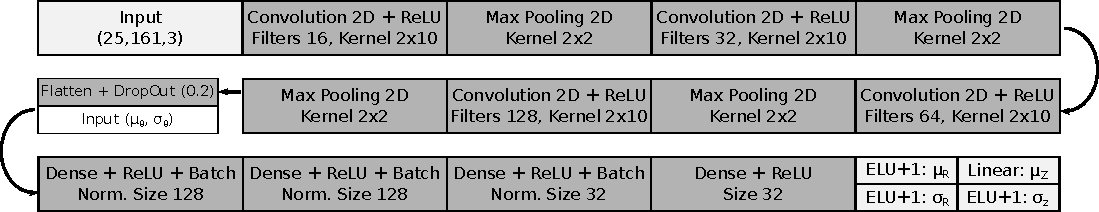
\includegraphics[scale=0.69]{figs2/DCN_RZ.pdf}
	\caption{\label{fig:network_RZ}Details of the closest point and interaction vertex network architecture.}
\end{figure}


\subsection{Energy}
\label{subsec:energy}

As described earlier, estimating the energy is particularly challenging for SL events, especially for track events, given their physical characteristics and the limited information available by a single line of the detector. Shower events are slightly better suited for energy reconstruction because of their physical topology. Moreover, the neutrino energy is directly inferred by $N$-fit in shower events, whereas for track events, the reconstructed energy by $N$-fit is limited to that of the secondary muon. This is due to the stochastic energy loss in neutrino interactions producing track events. The neutrino energy of track events for physics analyses can, however, be inferred indirectly, by combining $N$-fit energy reconstruction and the statistical properties of the interactions.

As a first approximation, we applied the same model architecture of the direction reconstruction to infer energy without further tuning. The energy reconstructions by that model presented very low accuracy. Reasons underlying the poor performance include that the secondary muon can escape the detector in track events, or that events could be very close or far away from the detector line in shower events. To better guide training in the $N$-fit energy reconstruction, we preselected events that we knew had good direction reconstruction (i.e., the events of the 50\% best $\sigma_\theta$), and that we knew that were close to the line (according to the $\{R,Z\}$ reconstruction). The specific cuts appear in expression (\ref{eq:cuts_tr}) for tracks, and in expression (\ref{eq:cuts_sh}) for showers.

\begin{equation}
\setlength{\jot}{10pt}
	\label{eq:cuts_tr}
	\begin{gathered}
		R_c \leq 50\,m~~~~Z_c \in (-150, 150)\,m~~~~\sigma_\theta\leq8.6^\circ\\
		\sigma_{R_c} \leq 4.3\,m~~~~\sigma_{Z_c} \leq 6.2\,m
	\end{gathered}
\end{equation}

\begin{equation}
\setlength{\jot}{10pt}
	\label{eq:cuts_sh}
	\begin{gathered}
		R_v \leq 50\,m~~~~Z_v \in (-150, 150)\,m~~~~\sigma_\theta\leq 14.9^\circ\\
		\sigma_{R_v} \leq 5.6\,m~~~~\sigma_{Z_v} \leq 3.3\,m
	\end{gathered}
\end{equation}

After training with these cuts, energy inference slightly improved. We considered this model as the \textit{benchmark} to evaluate further improvements, particularly that from indirect transfer learning through PCA-based knowledge distillation. In such approach, we aimed to exploit the relationship between the energy of the neutrino and all other physical parameters of the event processed by $N$-fit direction and distance models. We assumed that internal representations from those models could then benefit energy predictions. To test the hypothesis, neuron activations in hidden layers from the $\theta$ and $\{R,Z\}$ networks were taken as feature dimensions from which to infer events' energy. We disregarded, however, activations from the $\phi$ network for two main reasons, first due to the symmetry in $\{X,Y\}$, and second because of the low accuracy of $\phi$ estimations in SL events, compared to $\theta$ and $\{R,Z\}$ estimations.

We linearly transformed all feature dimensions, using the PCA, to rank components according to their variability. We then selected those most relevant features as inputs to a FFN trained to infer the energy as point predictions (\autoref{fig:network_e}). The final number of components, 63 features for the track branch and 68 for the shower branch, was determined applying the elbow rule, i.e., stopping incorporating more features once the cumulated variance reached a \textit{plateau}. Concurrently, we realized that inferring $\log (E)$ performed better than estimating $E$ directly, due to the large energy range of neutrino events (from 5 GeV up to 20 TeV).

In a subsequent phase aimed to further improve energy predictions for physics analyses, we designed a specialized FFN by feeding the model during training only with the 50\% best reconstructions from the original model shown in \autoref{fig:network_e}. In addition, this specialized FFN incorporated a MDN output layer to provide uncertainty estimation of energy predictions, as well as loss weighting factors to balance the impact of the non-uniform energy distribution.

\begin{figure}[htbp]
	\centering
	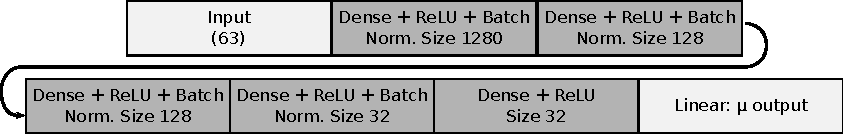
\includegraphics[scale=0.69]{figs2/NNEnergy.pdf}
	\caption{\label{fig:network_e}Details of the energy network architecture.}
\end{figure}

\subsection{Classification}
\label{subsec:class}

$N$-fit includes a neural network for track vs. shower classification, which leverages transfer learning from the specialized track and shower branches. It outputs the probability of an event to be a track ($P$), so the probability of being shower is $1-P$. To train, validate and test the classifier, we used a combined dataset made of 200,000 MC events, half of them representing track events ($\nu_\mu^{CC}$) and the other half representing shower events ($\nu_\mu^{NC}$, $\nu_e^{NC}$, $\nu_e^{CC}$). This new dataset, as well as the previous used in the training phase, are selected according to the $\chi^2$-fit SL criteria with no further refinement. All events were randomly sampled in a uniform manner covering the full period in which ANTARES collected data.

The \emph{control} network model for classification consisted of the same model architecture of the direction reconstruction without further tuning. Only the output was adjusted: a single neuron represented the probability of an event to be a track ($P$), using the sigmoid as its activation function. Given that track and shower events typically present different trace characteristics and that these traits were presumably present as internal representations in the convolutional layers of $N$-fit direction and distance reconstruction models, we decided to exploit this knowledge in a second, more sophisticated classifier endowed with TL. Specifically, we incorporated the convolutional blocks of the $\theta$, $\phi$ and $\{R,Z\}$ network models from both $N$-fit branches as frozen components that were plugged in parallel into a FFN. This network model also incorporated the reconstruction of the energy and its uncertainty from the networks specialized in track and shower events. The complete architecture is shown in \autoref{fig:network_class}.

\begin{figure}[htbp]
	\centering %width=1.\textwidth %scale=0.73
	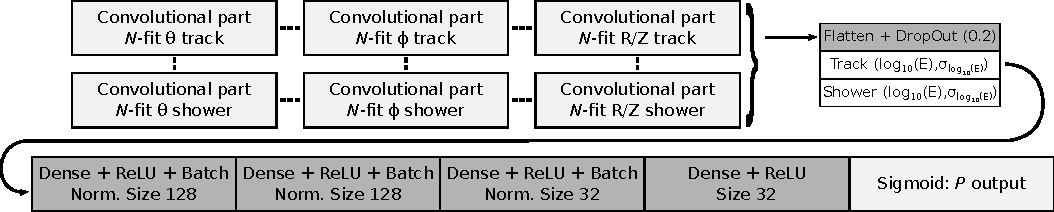
\includegraphics[scale=0.69]{figs2/DCN_class.pdf}
	\caption{\label{fig:network_class}Details of the classifier network architecture. All convolutional blocks are connected in parallel to the feed-forward part.}
\end{figure}

\subsection{Code implementation and computational efficiency}
\label{subsec:code}

All neural network models were implemented using the TensorFlow 2.4.1 framework, with model evaluation and analysis conducted in Python 3.9.15. The implementation relied on standard scientific computing libraries, including \texttt{NumPy 1.23.4}, \texttt{Scikit-learn 1.1.3}, and \texttt{Pandas 1.5.1}, along with several auxiliary packages.

Training times varied depending on network architecture. Specifically, direction and position networks required approximately 12 hours each to train, leveraging GPU acceleration via TensorFlow. Principal Component Analysis, applied separately to each branch (track and shower), required roughly 15 minutes per branch. The subsequent training of the energy reconstruction networks took between 5 and 15 minutes, being much faster than the spatial models primarily due to their lack of convolutional layers, which are typically the most computationally demanding components. Training the track vs. shower classifier, which reuses frozen convolutional layers transferred from the specialized branches, was comparatively lightweight, requiring only about 20 minutes. GPU-accelerated training was conducted on a workstation running KDE Neon 24.04, equipped with two NVIDIA Quadro RTX 8000 GPUs (TU102GL architecture, 64-bit interface), each of them having a 48 GB GDDR6 memory and supporting 672 GB/s memory bandwidth. % The system used the proprietary NVIDIA driver and was accessed via a KDE Neon 24.04 environment.

%All training and testing procedures were executed on a small server... \notaJGM{@Salva, ¿Puedes dar detalles del hardware, GPU, CPU, RAM, y software?}

The final application of the $N$-fit algorithm to ANTARES data was organized into three main phases: (i) reading the ANTARES data files, (ii) processing the raw data into the standardized $N$-fit input format, and (iii) performing the actual reconstruction. The first phase is common to any reconstruction pipeline and does not affect the evaluation of $N$-fit's computational performance. The image generation stage, where detector hits are transformed into 2D representations for network input, took on average 0.2 seconds per event. The complete reconstruction process required approximately 0.1 seconds per event. These estimates are based on the averaged processing times over 10,000 events, using conservative rounding to ensure upper-bound accuracy. In both cases, model parameters and dependencies were preloaded into memory cache, eliminating the overhead of repeated I/O operations during batch processing.

The whole application of $N$-fit to the ANTARES data was executed on the high-throughput computing (HTC) partition of the IN2P3 Computing Center, managed via the SLURM workload manager. The HTC partition consists of heterogeneous CPU-only nodes running Red Hat Enterprise Linux release 9.6 (64-bit). Most nodes are equipped with AMD EPYC 7302 16-core, EPYC 7453 28-core, or EPYC 9334 32-core processors, with memory per node ranging from 192~GB to over 1.2~TB. For our runs, a single CPU core and less than 2~GB of RAM were sufficient for efficient reconstruction inference. GPU resources were not required for deployment, although training leveraged TensorFlow's GPU acceleration when available.


%\notaSA{Dado que, como dice Juan, (1) los datos de ANTARES a nivel de hits están disponibles solo para la colaboración, y que (2) también existen limitaciones sobre código ANTARES, pero como (3) ANTARES ya ha concluido su labor, al menos en lo que respecta a la toma de nuevos datos; me parece que le deberíamos comentar a la comisión interna de revisión del manuscrito sobre la disponibilidad en abierto del (a) código y/o (b) los datos que se han usado, en algún repositorio público que podamos referenciar en el manuscrito; según su respuesta, las referencias se añadirían aquí, o no.}